\documentclass[border=4pt,varwidth=17cm]{standalone}
\usepackage{amsmath,amssymb,mathrsfs,mathtools}
\usepackage{tikz}
\usetikzlibrary{positioning,fit,backgrounds,arrows.meta}
\def\RR{{\mathbb R}}\def\eps{\varepsilon}\def\then{\Rightarrow}
\def\J{\mathcal{J}_L}\def\A{\mathcal{A}_{f,g}}\def\Sol{\mathcal{S}_{f,g}}
\def\limsup{\mathop{\overline{\lim}}}\def\liminf{\mathop{\underline{\lim}}}
\def\Of{{\sf (O$_f$)}}\def\Og{{\sf (O$_g$)}}
\def\Rv{{\sf (R$_{\rm v}$)}}\def\Rh{{\sf (R$_{\rm h}$)}}
\begin{document}


\scalebox{0.8}{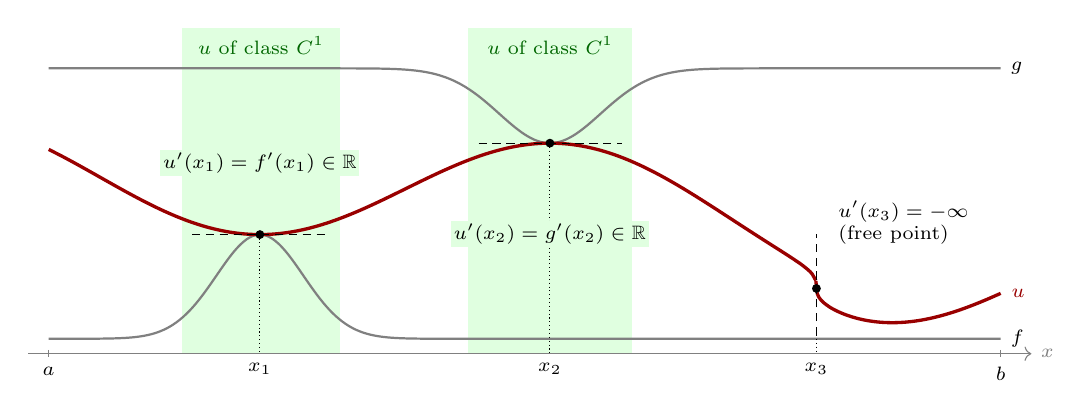
\begin{tikzpicture}[x=1.3cm, y=0.95cm, font=\scriptsize,
  declare function={S(\t)=-0.45*((\t<8) ? -1 : 1)*abs(\t-8)^(1/3);
    U(\t)=1.5+0.7*sin(deg(pi*(\t-4)/3))+S(\t);
    F(\t)=0.2+(1.5928-0.2)*exp(-((\t-2.5633)/0.6)^2);
    G(\t)=3.815-exp(-((\t-5.3965)/0.7)^2);}]
  % C^1 neighbourhoods of the contact points
  \fill[green!12] (1.8,0) rectangle (3.35,4.35);
  \fill[green!12] (4.6,0) rectangle (6.2,4.35);
  \node[green!40!black] at (2.575,4.12) {$u$ of class $C^1$};
  \node[green!40!black] at (5.4,4.12) {$u$ of class $C^1$};
  % axis and endpoints
  \draw[->, gray] (0.3,0) -- (10.1,0) node[right] {$x$};
  \draw[gray] (0.5,0.05) -- (0.5,-0.05) node[below, black] {$a$};
  \draw[gray] (9.8,0.05) -- (9.8,-0.05) node[below, black] {$b$};
  % obstacles
  \draw[thick, gray, domain=0.5:9.8, samples=150, smooth] plot (\x, {F(\x)}) node[right, black] {$f$};
  \draw[thick, gray, domain=0.5:9.8, samples=150, smooth] plot (\x, {G(\x)}) node[right, black] {$g$};
  % solution
  \draw[very thick, red!60!black, domain=0.5:7.995, samples=200, smooth] plot (\x, {U(\x)});
  \draw[very thick, red!60!black, domain=8.005:9.8, samples=100, smooth] plot (\x, {U(\x)}) node[right] {$u$};
  \draw[very thick, red!60!black] (7.995,{U(7.995)}) -- (8.005,{U(8.005)});
  % contact points
  \fill (2.5633,1.5928) circle (1.6pt);
  \draw[densely dashed] (1.9,{1.5928}) -- (3.25,{1.5928});
  \draw[densely dotted] (2.5633,1.5928) -- (2.5633,0) node[below] {$x_1$};
  \node[fill=green!12, inner sep=1pt] at (2.5633,2.55) {$u^\prime(x_1)=f^\prime(x_1)\in\RR$};
  \fill (5.3965,2.81495) circle (1.6pt);
  \draw[densely dashed] (4.7,2.81495) -- (6.1,2.81495);
  \draw[densely dotted] (5.3965,2.81495) -- (5.3965,0) node[below] {$x_2$};
  \node[fill=green!12, inner sep=1pt] at (5.3965,1.6) {$u^\prime(x_2)=g^\prime(x_2)\in\RR$};
  % singular free point
  \fill (8,{U(8.0001)}) circle (1.6pt);
  \draw[densely dashed] (8,0.25) -- (8,1.6);
  \draw[densely dotted] (8,0.25) -- (8,0) node[below] {$x_3$};
  \node[align=left, anchor=west] at (8.12,1.75) {$u^\prime(x_3)=-\infty$\\(free point)};
\end{tikzpicture}}


\end{document}
